\section{Distribution}
To distribute \doom, id software once again adopted the shareware model. A part of the game is given away for free (in the case of \doom, Episode 1) and players are encouraged to copy and give away this part. If they wanted the full game (with all weapons, monsters and maps) they had to pay for it.\\
\par
Only this time Jay Wilbur managed to get brick and mortar store on board with an offer they could not refuse.\\
\par
\fq{We told the retailers "we don't care if you make money off this shareware demo". "Move it. Move it in mass quantities." The retailers couldn't believe their ears, no one had ever told them not to pay royalties.
But Jay was insistent. "Take DOOM for nothing, keep the profit". My goal is distribution. DOOM is going to
be Wolfenstein on steroids, and I want it far and wide.
I want you to stack DOOM high. In fact, I want you to
do advertising for it, too, because you're going to make money off it. So take this money that you might have given me in royalties and use it to advertise the fact that you're selling DOOM.}{Jay}
\par
The shareware would find its way everywhere and well beyond game boxes. Book authors bundled it with their "Strategy guides". Magazine had to be wrapped in plastic bag to contain the two floppy disks it took to store the game.\\
\par
\fq{The challenge was: "How do we get Doom in the store? How do we get something free on shelves?\\
\par 
The idea was that the title screen of doom says "Suggested retail price \$9 dollars" on it and then we told the
companies that were already in the stores "if you put DOOM in the store in a box on the shelf you just keep all
the money. We don't want any of it just put it in a box and sell it".\\
\par 
Nutty, except that worked. It was everywhere. If you went into a CompUSA back then in 1994 you would see ten different boxes of doom and think they're all different games but they're all the same shareware game. Distributors ended up trying to make the best looking boxes to outperform their competitors because all they were allowed to sell was the shareware.}{John Romero}


\fullimage{endoom.png}\\%{Leaving the game displays instructions on how to buy it.}
\par
%Ideally, to make distribution as easy as possible, the game would have fitted on one 3\nicefrac{1}{2}-inch floppy disk. Even though 650 KiB floppy reader were fading out in favor of 1,440 KiB floppies, because of the volume of assets, DooM shareware still used two disks.\\
\par
\cfullimage{floppies.png}{Two floppies containing Doom shareware. Notice how they were in fact bundled with the book "Survivor's Strategies and Secrets"}
\par


\subsection{WAD archive: Where Are the Data}

Trivia: WAD was coined by Tom Halls. "Where's all the data?".\\
\pagebreak



\subsection{What's in the disk?}
INCLUDE A DOS DIS OF A FRESH INSTALL OF DOOM.
\par


\def\angle{0}
\def\radius{3}
\def\cyclelist{{"orange","blue","red","green"}}
\newcount\cyclecount \cyclecount=-1
\newcount\ind \ind=-1


\begin{figure}[H]
\centering
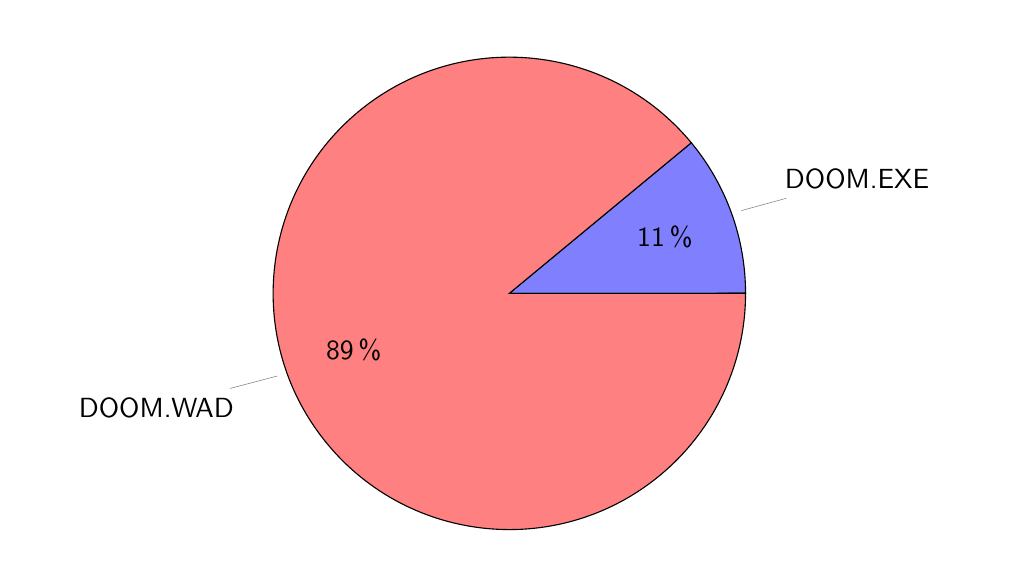
\begin{tikzpicture}[nodes = {font=\sffamily}]
  \node (a) at (6,0) {};
  \node (b) at (-6,0) {};
  \foreach \percent/\name in {
      11/DOOM.EXE,
      89/DOOM.WAD
    } {
      \ifx\percent\empty\else               % If \percent is empty, do nothing
        \global\advance\cyclecount by 1     % Advance cyclecount
        \global\advance\ind by 1            % Advance list index
        \ifnum3<\cyclecount                 % If cyclecount is larger than list
          \global\cyclecount=0              %   reset cyclecount and
          \global\ind=0                     %   reset list index
        \fi
        \pgfmathparse{\cyclelist[\the\ind]} % Get color from cycle list
        \edef\color{\pgfmathresult}         %   and store as \color
        % Draw angle and set labels
        \draw[fill={\color!50},draw={black}] (0,0) -- (\angle:\radius)
          arc (\angle:\angle+\percent*3.6:\radius) -- cycle;
        \node at (\angle+0.5*\percent*3.6:0.7*\radius) {\percent\,\%};
        \node[pin=\angle+0.5*\percent*3.6:\name]
          at (\angle+0.5*\percent*3.6:\radius) {};
        \pgfmathparse{\angle+\percent*3.6}  % Advance angle
        \xdef\angle{\pgfmathresult}         %   and store in \angle
      \fi
      
    };
\end{tikzpicture}
\end{figure}



\par
\begin{figure}[H]
\centering
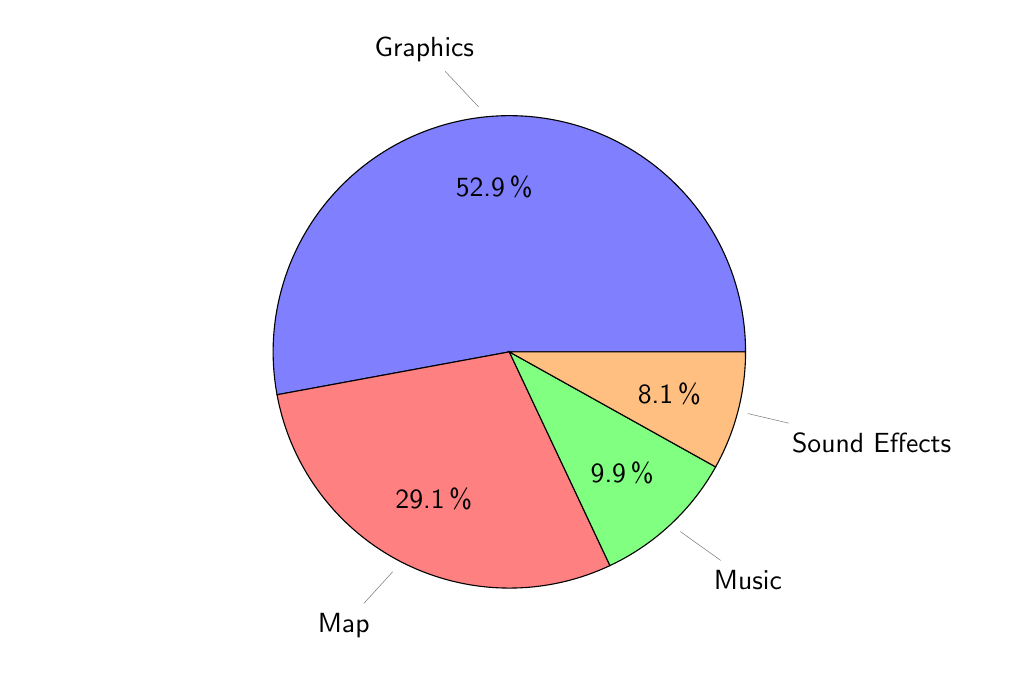
\begin{tikzpicture}[nodes = {font=\sffamily}]
\node (a) at (6,0) {};
  \node (b) at (-6,0) {};
  \foreach \percent/\name in {
      52.9/Graphics,
      29.1/Map,
       9.9/Music,
       8.1/{Sound Effects},
    } {
      \ifx\percent\empty\else               % If \percent is empty, do nothing
        \global\advance\cyclecount by 1     % Advance cyclecount
        \global\advance\ind by 1            % Advance list index
        \ifnum3<\cyclecount                 % If cyclecount is larger than list
          \global\cyclecount=0              %   reset cyclecount and
          \global\ind=0                     %   reset list index
        \fi
        \pgfmathparse{\cyclelist[\the\ind]} % Get color from cycle list
        \edef\color{\pgfmathresult}         %   and store as \color
        % Draw angle and set labels
        \draw[fill={\color!50},draw={black}] (0,0) -- (\angle:\radius)
          arc (\angle:\angle+\percent*3.6:\radius) -- cycle;
        \node at (\angle+0.5*\percent*3.6:0.7*\radius) {\percent\,\%};
        \node[pin=\angle+0.5*\percent*3.6:\name]
          at (\angle+0.5*\percent*3.6:\radius) {};
        \pgfmathparse{\angle+\percent*3.6}  % Advance angle
        \xdef\angle{\pgfmathresult}         %   and store in \angle
      \fi
    };
\end{tikzpicture}
\end{figure}
